%%%%%%%%%%%%%%%%%%%%%%%%%%%%%%%%%%%%%%%%%
% Beamer Presentation
% LaTeX Template
% Version 1.0 (10/11/12)
%
% This template has been downloaded from:
% http://www.LaTeXTemplates.com
%
% License:
% CC BY-NC-SA 3.0 (http://creativecommons.org/licenses/by-nc-sa/3.0/)
%
%%%%%%%%%%%%%%%%%%%%%%%%%%%%%%%%%%%%%%%%%

%----------------------------------------------------------------------------------------
%	PACKAGES AND THEMES
%----------------------------------------------------------------------------------------

%\documentclass[UTF8,aspectratio=169,14pt]{ctexbeamer}
\documentclass[UTF8,aspectratio=169]{ctexbeamer}
\usepackage{hyperref}
\hypersetup{
	colorlinks=true,
	linkcolor=red,
	anchorcolor=blue,
	citecolor=green
}

\mode<presentation> {
	
	% The Beamer class comes with a number of default slide themes
	% which change the colors and layouts of slides. Below this is a list
	% of all the themes, uncomment each in turn to see what they look like.
	
	%\usetheme{default}
	%\usetheme{AnnArbor}
	%\usetheme{Antibes}
	%\usetheme{Bergen}
	%\usetheme{Berkeley}
	%\usetheme{Berlin}
	%\usetheme{Boadilla}
	%\usetheme{CambridgeUS}
	%\usetheme{Copenhagen}
	%\usetheme{Darmstadt}
	%\usetheme{Dresden}
	%\usetheme{Frankfurt}
	%\usetheme{Goettingen}
	%\usetheme{Hannover}
	%\usetheme{Ilmenau}
	%\usetheme{JuanLesPins}
	%\usetheme{Luebeck}
	\usetheme{Madrid}
	%\usetheme{Malmoe}
	%\usetheme{Marburg}
	%\usetheme{Montpellier}
	%\usetheme{PaloAlto}
	%\usetheme{Pittsburgh}
	%\usetheme{Rochester}
	%\usetheme{Singapore}
	%\usetheme{Szeged}
	%\usetheme{Warsaw}
	
	% As well as themes, the Beamer class has a number of color themes
	% for any slide theme. Uncomment each of these in turn to see how it
	% changes the colors of your current slide theme.
	
	%\usecolortheme{albatross}
	%\usecolortheme{beaver}
	%\usecolortheme{beetle}
	%\usecolortheme{crane}
	%\usecolortheme{dolphin}
	%\usecolortheme{dove}
	%\usecolortheme{fly}
	%\usecolortheme{lily}
	%\usecolortheme{orchid}
	%\usecolortheme{rose}
	%\usecolortheme{seagull}
	%\usecolortheme{seahorse}
	%\usecolortheme{whale}
	%\usecolortheme{wolverine}
	
	%\setbeamertemplate{footline} % To remove the footer line in all slides uncomment this line
	%\setbeamertemplate{footline}[page number] % To replace the footer line in all slides with a simple slide count uncomment this line
	
	%\setbeamertemplate{navigation symbols}{} % To remove the navigation symbols from the bottom of all slides uncomment this line
}

\usepackage{graphicx} % Allows including images
\graphicspath{{./figs/}}
\usepackage{booktabs} % Allows the use of \toprule, \midrule and \bottomrule in tables
\usepackage{longtable}
\usepackage{listings}
\usepackage{xcolor}
\lstset{numbers=left, %设置行号位置
	numberstyle=\tiny, %设置行号大小
	keywordstyle=\color{blue}, %设置关键字颜色
	commentstyle=\color[cmyk]{1,0,1,0}, %设置注释颜色
	frame=single, %设置边框格式
	escapeinside=``, %逃逸字符(1左面的键),用于显示中文
	%breaklines, %自动折行
	extendedchars=false, %解决代码跨页时,章节标题,页眉等汉字不显示的问题
	xleftmargin=2em,xrightmargin=2em, aboveskip=1em, %设置边距
	tabsize=4, %设置tab空格数
	showspaces=false %不显示空格
}
% Fonts
% \usepackage{libertine}
% \setmonofont{Courier}
\setCJKsansfont[ItalicFont=Noto Serif CJK SC Black, BoldFont=Noto Sans CJK SC Black]{Noto Sans CJK SC}
\setmainfont[Ligatures={Common,TeX}]{Linux  Libertine O}
\setmonofont[SmallCapsFont={Latin Modern Mono Caps}]{Latin Modern Mono Light}
\setsansfont{Linux Biolinum O}

\logo{
\includegraphics[width=0.55cm,height=0.55cm]{../../thcs-logo.png}}

%----------------------------------------------------------------------------------------
%	TITLE PAGE
%----------------------------------------------------------------------------------------

\title[第14讲]{第14讲: Concurrency in OS Kernel} % The short title appears at the bottom of every slide, the full title is only on the title page
\subtitle{第三节:Scalable Concurrency -- RCU}
\author{陈渝} % Your name
\institute[清华大学] % Your institution as it will appear on the bottom of every slide, may be shorthand to save space
{
	清华大学计算机系 \\ % Your institution for the title page
	\medskip
	\textit{yuchen@tsinghua.edu.cn} % Your email address
}
\date{\today} % Date, can be changed to a custom dateC++ memory order



\begin{document}

\begin{frame}
\titlepage % Print the title page as the first slide
\end{frame}
    
%\begin{frame}
%\frametitle{提纲} % Table of contents slide, comment this block out to remove it
%\tableofcontents % Throughout your presentation, if you choose to use \section{} and \subsection{} commands, these will automatically be printed on this slide as an overview of your presentation
%\end{frame}
%
%%----------------------------------------------------------------------------------------
%%	PRESENTATION SLIDES
%%----------------------------------------------------------------------------------------
%

%----------------------------------------------
%-------------------------------------------------
\begin{frame}
    \frametitle{Resource}
    
    
    

	\begin{columns}
    
    \begin{column}{.5\textwidth}
        \centering
        
        
\includegraphics[width=.7\textwidth]{book-cpp-concurrency-in-action}
        
    \end{column}
    
    \begin{column}{.5\textwidth}
        
      
\includegraphics[width=.7\textwidth]{perfbook}
       
        
    \end{column}
    
    
\end{columns}
    
    \tiny Reference:
    
    "Is Parallel Programming Hard, And, If So, What Can You Do About It?",Paul McKenney;\\
    "C++Concurrency in Action", ANTHONY WILLIAMS; \\
    "CS510 - Advanced Topics in Concurrency", Jonathan Walpole;
    Adam Belay from MIT PDOS
    
%    http://www2.rdrop.com/users/paulmck/RCU/
%    https://lwn.net/Articles/262464/
\end{frame}

%----------------------------------------------
\begin{frame}[fragile]
    \frametitle{RCU}
    \Large
    Motivation
    \begin{itemize}
    \item Modern CPUs are predominantly multicore
    \item Applications rely heavily on kernel for networking,
    filesystem, etc.
    \item If kernel can’t scale across many cores, applications
    that rely on it won’t scale either
    \item Have to be able to execute system calls in parallel
\end{itemize}
\end{frame}
%----------------------------------------------
\begin{frame}[fragile]
    \frametitle{RCU}
    \Large
    Problem is sharing
    \begin{itemize}
        \item OS maintains many data structures
        \item They depend on locks to maintain invariants
        \item Applications may contend on locks, limiting
        scalability
        
    \end{itemize}
    
\end{frame}

%----------------------------------------------
\begin{frame}[fragile]
    \frametitle{RCU}
    \Large
    Read-heavy data structures
    
    Kernels often have data that is read much more
    often than it is modified
   
    \begin{itemize}
        \item Network tables: routing, ARP
        \item File descriptor arrays
        \item  system call state
    \end{itemize}
    
\end{frame}

%----------------------------------------------
\begin{frame}[fragile]
    \frametitle{RCU}
    \Large
   Goals
    
    \begin{itemize}
        \item Concurrent reads even during updates
        \item Low space overhead
        \item Low execution overhead
    \end{itemize}
    
\end{frame}


%----------------------------------------------
\begin{frame}[fragile]
    \frametitle{RCU}
    \Large
    Idea: Read-copy update (RCU)
    \begin{itemize}
        \item  Readers just access objects directly (no locks)
        \item  Writers make a copy of object, change it, then
        update the pointer to the new copy
    \end{itemize}
    \centering
    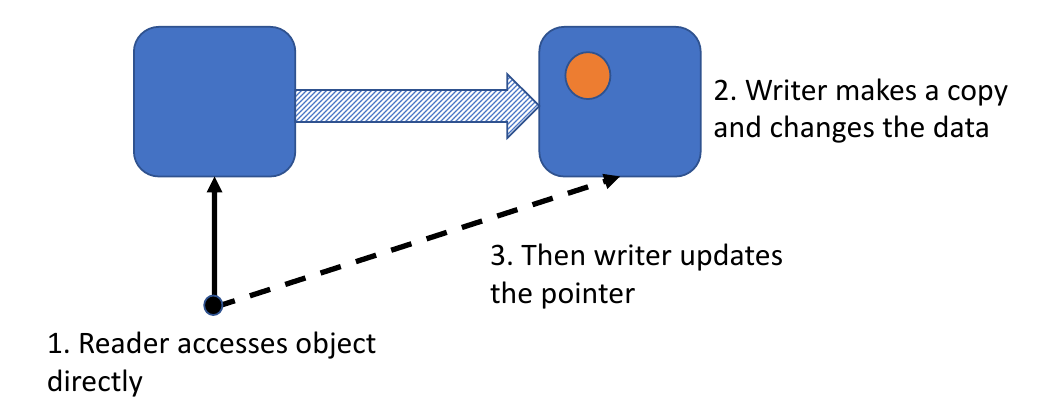
\includegraphics[width=.7\textwidth]{rcu}
\end{frame}

%----------------------------------------------
\begin{frame}[fragile]
    \frametitle{RCU}
    \Large
    Three fundamental mechanisms
    \begin{itemize}
        \item  Publish-Subscribe Mechanism (for insertion) 
        \item  Wait For Pre-Existing RCU Readers to Complete (for deletion) 
        \item Maintain Multiple Versions of Recently Updated Objects (for readers) 
    \end{itemize}
    \centering
    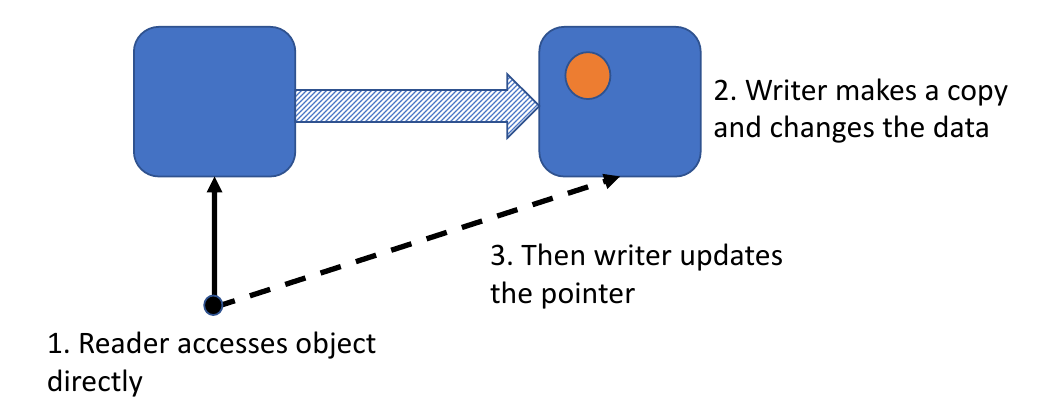
\includegraphics[width=.7\textwidth]{rcu}
    
    
%    在RCU的实现过程中,我们主要解决以下问题:
%    
%    1,在读取过程中,另外一个线程删除了一个节点。删除线程可以把这个节点从链表中移除,但它不能直接销毁这个节点,必须等到所有的读取线程读取完成以后,才进行销毁操作。RCU中把这个过程称为宽限期(Grace period)。
%    
%    2,在读取过程中,另外一个线程插入了一个新节点,而读线程读到了这个节点,那么需要保证读到的这个节点是完整的。这里涉及到了发布-订阅机制(Publish-Subscribe Mechanism)。
%    
%    3, 保证读取链表的完整性。新增或者删除一个节点,不至于导致遍历一个链表从中间断开。但是RCU并不保证一定能读到新增的节点或者不读到要被删除的节点。
\end{frame}


%----------------------------------------------
\begin{frame}[fragile]
    \frametitle{RCU -- Publish-Subscribe Mechanism}
    \Large
    One key attribute of RCU is the ability to safely scan data, even though that data is being modified concurrently.
    
\small
    \begin{block}{}
    \begin{verbatim}
1 struct foo {
2   int a;
3   int b;
4   int c;
5 };
6 struct foo *gp = NULL; ......
10 p = kmalloc(sizeof(*p), GFP_KERNEL);
11 p->a = 1;
12 p->b = 2;
13 p->c = 3;
14 gp = p;
\end{verbatim}
\end{block}  
\end{frame}


%----------------------------------------------
\begin{frame}[fragile]
    \frametitle{RCU -- Publish-Subscribe Mechanism}
    \Large
The rcu\_assign\_pointer() would publish the new structure, forcing both the compiler and the CPU to execute the assignment to gp after the assignments to the fields referenced by p. 
    
    \small
    \begin{block}{}
        \begin{verbatim}
1 struct foo {
2   int a;
3   int b;
4   int c;
5 };
6 struct foo *gp = NULL; ......
10 p = kmalloc(sizeof(*p), GFP_KERNEL);
11 p->a = 1;
12 p->b = 2;
13 p->c = 3;
14 rcu_assign_pointer(gp, p);
        \end{verbatim}
    \end{block}  
\end{frame}

%----------------------------------------------
\begin{frame}[fragile]
    \frametitle{RCU -- Publish-Subscribe Mechanism}
    \Large
    However, it is not sufficient to only enforce ordering at the updater, as the reader must enforce proper ordering as well.
    
    \small
    \begin{block}{}
        \begin{verbatim}
1 p = gp;
2 if (p != NULL) {
3   do_something_with(p->a, p->b, p->c);
4 }
        \end{verbatim}
    \end{block}  

\Large
the DEC Alpha CPU and value-speculation compiler optimizations can, believe it or not, cause the values of p->a, p->b, and p->c to be fetched before the value of p!
\end{frame}


%----------------------------------------------
\begin{frame}[fragile]
    \frametitle{RCU -- Publish-Subscribe Mechanism}
    \Large
    The rcu\_dereference() primitive uses whatever memory-barrier instructions and compiler directives are required for this purpose: 
    
    \small
    \begin{block}{}
        \begin{verbatim}
1 rcu_read_lock();
2 p = rcu_dereference(gp);
3 if (p != NULL) {
4   do_something_with(p->a, p->b, p->c);
5 }
6 rcu_read_unlock();
        \end{verbatim}
    \end{block}  
    
    \normalsize
The rcu\_dereference() primitive can thus be thought of as subscribing to a given value of the specified pointer, guaranteeing that subsequent dereference operations will see any initialization that occurred before the corresponding publish (rcu\_assign\_pointer()) operation. 
\end{frame}


%----------------------------------------------
\begin{frame}[fragile]
    \frametitle{RCU -- Publish-Subscribe Mechanism}
%    \Large
    \centering
    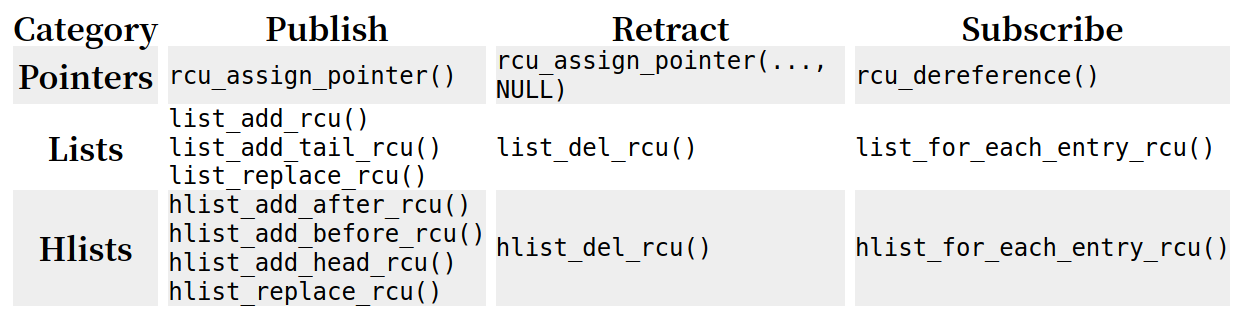
\includegraphics[width=1.\textwidth]{rcu-api}
\end{frame}


%----------------------------------------------
\begin{frame}[fragile]
    \frametitle{RCU -- Wait For Pre-Existing RCU Readers to Complete}
    \Large
    In its most basic form, RCU is a way of waiting for things to finish. 
    
    \centering
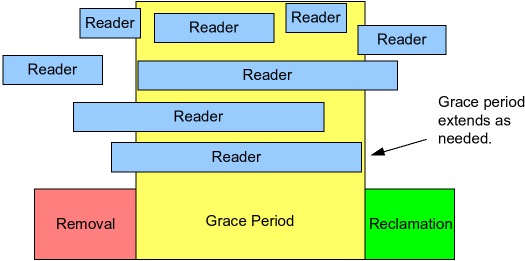
\includegraphics[width=.8\textwidth]{rcu-wait}
\end{frame}



%----------------------------------------------
\begin{frame}[fragile]
    \frametitle{RCU -- Wait For Pre-Existing RCU Readers to Complete}
    \Large
RCU to wait for readers: 
\begin{itemize}
    \item  Make a change, for example, replace an element in a linked list. 
    \item  Wait for all pre-existing RCU read-side critical sections to completely finish (for example, by using the synchronize\_rcu() primitive). The key observation here is that subsequent RCU read-side critical sections have no way to gain a reference to the newly removed element. 
    \item Clean up, for example, free the element that was replaced above.  
\end{itemize}
\end{frame}


%----------------------------------------------
\begin{frame}[fragile]
    \frametitle{RCU -- Wait For Pre-Existing RCU Readers to Complete}
    
    \small
    \begin{block}{}
        \begin{verbatim}
1 struct foo {
2   struct list_head list;
3   int a, b, c;
6 };
7 LIST_HEAD(head); ...
11 p = search(head, key);
12 if (p == NULL) {
13   /* Take appropriate action, unlock, and return. */
14 }
15 q = kmalloc(sizeof(*p), GFP_KERNEL);
16 *q = *p; q->b = 2;  q->c = 3;
19 list_replace_rcu(&p->list, &q->list);
20 synchronize_rcu();
21 kfree(p);
\end{verbatim}
\end{block}  
\large
Lines 19, 20, and 21 implement the three steps called out above.
\end{frame}

%----------------------------------------------
\begin{frame}[fragile]
    \frametitle{RCU -- Wait For Pre-Existing RCU Readers to Complete}
    \large
    RCU Classic's synchronize\_rcu() can conceptually be as simple as the following:
%    \small
    \begin{block}{}
        \begin{verbatim}
1 for_each_online_cpu(cpu)
2   run_on(cpu);
        \end{verbatim}
    \end{block}  
    \large

\end{frame}
%----------------------------------------------
\begin{frame}[fragile]
    \frametitle{RCU -- Wait For Pre-Existing RCU Readers to Complete}
    \Large
    RCU  readers: 
    \begin{itemize}
        \item   the rcu\_read\_lock() and rcu\_read\_unlock() primitives that delimit RCU read-side critical sections don't even generate any code in non-CONFIG\_PREEMPT kernels! 
        \item RCU Classic read-side critical sections delimited by rcu\_read\_lock() and rcu\_read\_unlock() are not permitted to block or sleep.
    \end{itemize}
\end{frame}


%----------------------------------------------
\begin{frame}[fragile]
    \frametitle{RCU -- Maintain Multiple Versions of Recently Updated Objects}
    \Large
    Example 1: Maintaining Multiple Versions During Deletion
%    \small
\begin{block}{}
    \begin{verbatim}
1 p = search(head, key);
2 if (p != NULL) {
3   list_del_rcu(&p->list);
4   synchronize_rcu();
5   kfree(p);
6 }
    \end{verbatim}
\end{block} 
\end{frame}


%----------------------------------------------
\begin{frame}[fragile]
    \frametitle{RCU -- Maintain Multiple Versions of Recently Updated Objects}
    \Large
    Example 1: Maintaining Multiple Versions During Deletion \\
    
    The initial state of the list, including the pointer p, is as follows. 
    %    \small
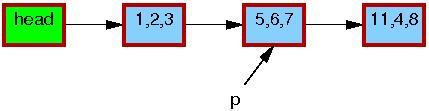
\includegraphics[width=.8\textwidth]{rcu-multiver-ex1}
\end{frame}

%----------------------------------------------
\begin{frame}[fragile]
    \frametitle{RCU -- Maintain Multiple Versions of Recently Updated Objects}
    \Large
    Example 1: Maintaining Multiple Versions During Deletion \\
    
    After the list\_del\_rcu() on line 3 has completed, the 5,6,7 element has been removed from the list, as shown below. 
    %    \small
    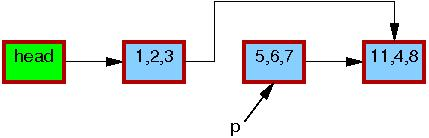
\includegraphics[width=.8\textwidth]{rcu-multiver-ex2}
\end{frame}

%----------------------------------------------
\begin{frame}[fragile]
    \frametitle{RCU -- Maintain Multiple Versions of Recently Updated Objects}
    \Large
    Example 1: Maintaining Multiple Versions During Deletion \\
    
    once the synchronize\_rcu() on line 4 completes, so that all pre-existing readers are guaranteed to have completed, there can be no more readers referencing this element, as indicated by its black border below.
    %    \small
    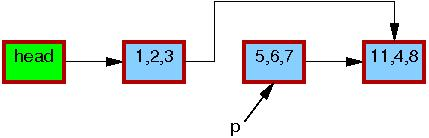
\includegraphics[width=.8\textwidth]{rcu-multiver-ex2}
\end{frame}

%----------------------------------------------
\begin{frame}[fragile]
    \frametitle{RCU -- Maintain Multiple Versions of Recently Updated Objects}
    \Large
    Example 1: Maintaining Multiple Versions During Deletion \\
    
    At this point, the 5,6,7 element may safely be freed, as shown below: 
    %    \small
    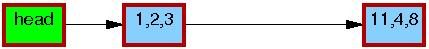
\includegraphics[width=.8\textwidth]{rcu-multiver-ex3}
\end{frame}


%----------------------------------------------
\begin{frame}[fragile]
    \frametitle{RCU -- Maintain Multiple Versions of Recently Updated Objects}
    \Large
    Example 2: Maintaining Multiple Versions During Replacement
    %    \small
    \begin{block}{}
        \begin{verbatim}
1 q = kmalloc(sizeof(*p), GFP_KERNEL);
2 *q = *p;
3 q->b = 2;
4 q->c = 3;
5 list_replace_rcu(&p->list, &q->list);
6 synchronize_rcu();
7 kfree(p);
        \end{verbatim}
    \end{block} 
\end{frame}

%----------------------------------------------
\begin{frame}[fragile]
    \frametitle{RCU -- Maintain Multiple Versions of Recently Updated Objects}
    \Large
    Example 2: Maintaining Multiple Versions During Replacement \\
    
    The initial state of the list, including the pointer p, is as follows. 
    %    \small
    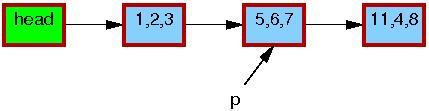
\includegraphics[width=.8\textwidth]{rcu-multiver-ex1}
\end{frame}

%----------------------------------------------
\begin{frame}[fragile]
    \frametitle{RCU -- Maintain Multiple Versions of Recently Updated Objects}
    \Large
    Example 2: Maintaining Multiple Versions During Replacement \\
    
    Line 1 kmalloc()s a replacement element, as follows: 
    %    \small
    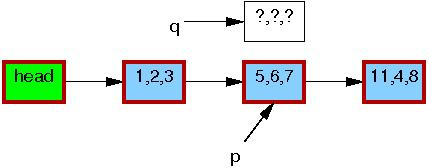
\includegraphics[width=.8\textwidth]{rcu-multiver-ex4}
\end{frame}


%----------------------------------------------
\begin{frame}[fragile]
    \frametitle{RCU -- Maintain Multiple Versions of Recently Updated Objects}
    \Large
    Example 2: Maintaining Multiple Versions During Replacement \\
    
    Line 2 copies the old element to the new one:  
    %    \small
    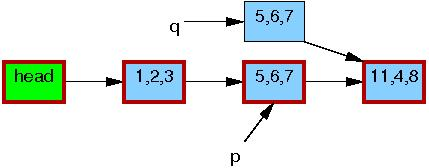
\includegraphics[width=.8\textwidth]{rcu-multiver-ex5}
\end{frame}

%----------------------------------------------
\begin{frame}[fragile]
    \frametitle{RCU -- Maintain Multiple Versions of Recently Updated Objects}
    \Large
    Example 2: Maintaining Multiple Versions During Replacement \\
    
    Line 3 updates q->b to the value "2":  
    %    \small
    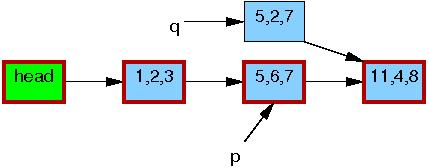
\includegraphics[width=.8\textwidth]{rcu-multiver-ex6}
\end{frame}


%----------------------------------------------
\begin{frame}[fragile]
    \frametitle{RCU -- Maintain Multiple Versions of Recently Updated Objects}
    \large
    Example 2: Maintaining Multiple Versions During Replacement \\
    
    Now, line 5 does the replacement, so that the new element is finally visible to readers. At this point, as shown below, we have two versions of the list. 
    %    \small
    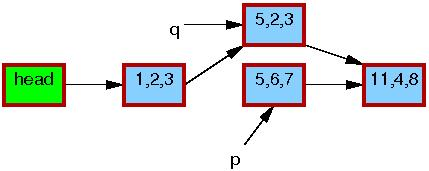
\includegraphics[width=.8\textwidth]{rcu-multiver-ex7}
\end{frame}


%----------------------------------------------
\begin{frame}[fragile]
    \frametitle{RCU -- Maintain Multiple Versions of Recently Updated Objects}
    \large
    Example 2: Maintaining Multiple Versions During Replacement \\
    
After the synchronize\_rcu() on line 6 returns, a grace period will have elapsed, and so all reads that started before the list\_replace\_rcu() will have completed.
    %    \small
    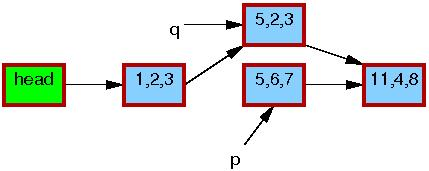
\includegraphics[width=.8\textwidth]{rcu-multiver-ex7}
\end{frame}

%----------------------------------------------
\begin{frame}[fragile]
    \frametitle{RCU -- Maintain Multiple Versions of Recently Updated Objects}
    \large
    Example 2: Maintaining Multiple Versions During Replacement \\
    
    After the kfree() on line 7 completes, the list will appear as follows: 
    %    \small
    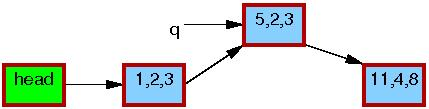
\includegraphics[width=.8\textwidth]{rcu-multiver-ex8}
\end{frame}

%----------------------------------------------
\begin{frame}[fragile]
    \frametitle{Conclusion}
    \Large
    \begin{itemize}
    \item RCU enables zero-cost read-only access at the
    expense of slightly more expensive updates
    \item Very useful for read-mostly data (extremely common in
    kernels)
\end{itemize}
\end{frame}

%----------------------------------------------
%----------------------------------------------
\end{document}